\documentclass[12pt, letterpaper]{article}
\usepackage[utf8]{inputenc}
\usepackage{geometry}
\geometry{letterpaper, margin=1in}
\usepackage{graphicx}
\usepackage{amsmath}
\usepackage{amssymb}
\usepackage{hyperref}
\usepackage{cite}
\usepackage{algorithm}
\usepackage{algpseudocode}
\usepackage{bm}
\usepackage{tikz}
\usetikzlibrary{shapes.geometric, arrows.meta, positioning, fit, calc}
\usepackage{booktabs}
\usepackage{multirow}

\title{Pareto Set Learning for Autonomous Highway Navigation}
\author{
  Ravichandra Parvatham (ID: 122182264) \and
  Aadit Pratik Maniar (ID: 121334749) \and
  Gautam Bulusu (ID: 121968470)
}
\date{
  MSML 604 Introduction to Optimization\\
  University of Maryland, College Park
}

\begin{document}

\maketitle

\begin{abstract}
Autonomous Vehicles (AVs) must navigate inherently conflicting objectives: safety, speed, and comfort. Traditional methods rely on fixed scalarization, which fails to capture the diversity of optimal driving behaviors. This project proposes the application of LibMOON, a gradient-based multi-objective optimization library, to the \texttt{highway-env} simulation. By utilizing Pareto Set Learning (PSL), we aim to learn a Pareto set of optimal policies, allowing for dynamic adjustment of driving styles without the need for retraining. The project repository is available at: \url{https://github.com/aaditManiar/autonomous-driving-psl}.
\end{abstract}

\section{Introduction \& Related Literature}

\subsection{Motivation and Problem Context}
Autonomous driving in high-speed highway environments necessitates a delicate balance between competing goals. A vehicle prioritizing safety may become overly conservative, hindering traffic flow, while a focus on speed may lead to aggressive maneuvers that compromise passenger comfort and safety margins. The fundamental challenge lies in the fact that these objectives are non-commensurable and vary based on context (e.g., weather, traffic density, or passenger preference). Current control systems typically collapse these objectives into a single scalar cost function via manual weight tuning. Such approaches are computationally expensive to re-tune and fail to represent the Pareto Front—the set of solutions where no objective can be improved without degrading another.

The motivation for this study is to move beyond static, "one-size-fits-all" autonomous driving policies. Real-world deployment requires flexibility; for instance, an AV may need to switch from an "Efficiency Mode" for daily commuting to a "Safety-First Mode" during adverse weather conditions. By applying Pareto Set Learning (PSL) solvers from the recently introduced LibMOON library to the \texttt{highway-env} environment, we bridge the gap between theoretical multi-objective optimization (MOO) and sequential decision-making. While LibMOON has shown promise on synthetic benchmarks, its performance in dynamic, high-stakes robotic simulations remains largely unstudied. This project provides a critical evaluation of gradient-based MOO for real-time autonomous control.

\subsection{Related Literature}

\textbf{Reinforcement Learning and Autonomous Driving:} 
Deep Reinforcement Learning (DRL) has emerged as a dominant paradigm for sequential decision-making in autonomous navigation \cite{kiran2021deep}. These sequential tasks often leverage the Actor-Critic framework, initially formalized by Konda and Tsitsiklis \cite{konda2000actor}, which separates the policy (actor) from the expected return estimation (critic) to stabilize gradient updates. However, standard RL formulations typically rely on a single scalar reward, which struggles to encapsulate the multifaceted, conflicting nature of real-world driving metrics. To address this, recent work has increasingly formulated autonomous driving as a Multi-Objective Markov Decision Process (MOMDP), enabling the simultaneous consideration of various driving goals \cite{agbaje2024neuroaction}.

\textbf{Multi-Objective Optimization (MOO) \& MORL:} 
Multi-Objective RL (MORL) extends standard RL by vectorizing the reward signal \cite{hayes2022practical}. The goal in MORL is to construct a diverse set of optimal policies that collectively form a Pareto set, allowing for policies to be selected based on specific out- and in-car scenarios. While classic evolutionary algorithms like NSGA-II \cite{deb2002fast} are highly effective for general MOO problems, they are often computationally prohibitive when scaling to the millions of parameters typical in deep neural networks.

\textbf{Pareto Set Learning (PSL) \& Hypernetworks:} 
Instead of repeatedly solving scalarized instances or employing inefficient repetitive retraining to find discrete trade-offs, Pareto Set Learning (PSL) aims to approximate the entire continuous Pareto front in a single training process. Navon et al. \cite{navon2020learning} demonstrated that Preference Hypernetworks (PHNs) can map a continuous preference vector directly to the weights of a target model. More recently, frameworks like PSL-MORL have been proposed to harness the generation capability of hypernetworks within reinforcement learning, producing personalized policy network parameters for each preference vector and achieving dense coverage of the Pareto front \cite{liu2025pareto}. 

\textbf{Gradient-Based Optimization Libraries:} 
Scaling PSL to complex neural architectures requires specialized tooling. LibMOON \cite{zhang2024libmoon} was introduced as a PyTorch-based framework specifically designed to support state-of-the-art gradient-based MOO algorithms. By efficiently utilizing higher-order information from objectives, LibMOON circumvents the scalability limitations of zeroth-order evolutionary methods, making it highly suitable for deep MORL applications.

\textbf{Simulation Environments:} 
Validating multi-objective decision-making algorithms requires customizable, dynamic simulation environments. The \texttt{highway-env} framework \cite{leurent2018highway} provides a streamlined platform for simulating diverse highway and intersection traffic scenarios. It exposes vectorized kinematic states and customizable reward functions, making it an ideal testbed for evaluating the continuous control and trade-off balancing required by MORL and PSL algorithms.

\section{Problem Formulation}

\subsection{Multi-Objective Markov Decision Process}
We formulate highway navigation as a Multi-Objective Markov Decision Process (MOMDP) \cite{roijers2013survey,hayes2022practical}, defined by the tuple $\mathcal{M}=\langle \mathcal{S}, \mathcal{A}, \mathcal{P}, \bm{r}, \gamma \rangle$, where the conventional scalar reward is replaced with a vector-valued cost signal $\bm{r} : \mathcal{S} \times \mathcal{A} \to \mathbb{R}^m$ with $m = 3$. The state space $\mathcal{S}$ is realised through the kinematic observation produced by \texttt{highway-env} \cite{leurent2018highway}: a $5 \times 5$ matrix encoding the ego vehicle and its four nearest neighbours, with features $[p, x, y, v_x, v_y]$ where $p$ is a presence indicator and the spatial features are normalised relative to the ego frame. The action space $\mathcal{A}$ uses the \texttt{DiscreteMetaAction} interface with five high-level options: $\{\textsc{Lane\_Left}, \textsc{Idle}, \textsc{Lane\_Right}, \textsc{Faster}, \textsc{Slower}\}$. The agent acts at $f_{\pi} = 2~\text{Hz}$, yielding a control timestep of $\Delta t = 0.5$ s, while the underlying simulation runs at $15$ Hz to integrate continuous dynamics.

\subsection{Per-Step Cost Vector}
At every decision step $t$ we evaluate three normalised cost components $\bm{r}_t = [r_t^{\text{safe}}, r_t^{\text{speed}}, r_t^{\text{cmft}}]^{\top} \in [0,1]^3$, all of which are minimised (lower is better). This sign convention aligns with LibMOON's \cite{zhang2024libmoon} optimisation interface, which expects costs rather than rewards.

\paragraph{Safety.}
We use a smooth surrogate of the inverse Time-to-Collision (iTTC), a standard surrogate safety measure in vehicular research \cite{vogel2003ttc}. Let $g$ be the longitudinal gap to the nearest in-lane lead vehicle and $\Delta v$ the closing rate. Define
\begin{equation}
    \mathrm{TTC}(s_t) =
    \begin{cases}
        g/\Delta v & \Delta v > 0,\\
        +\infty & \text{otherwise.}
    \end{cases}
\end{equation}
Letting $\tau_{\!*}$ denote a safety reference horizon, we evaluate
\begin{equation}
    \mathrm{iTTC}(s_t) = \mathrm{clip}\!\Big(\tfrac{\tau_{\!*}}{\mathrm{TTC}(s_t)}, 0, 1\Big), \qquad \tau_{\!*} = 5~\text{s}.
\end{equation}
This formulation produces a strictly positive gradient signal whenever the ego is closing on a leader, even at large TTC. Earlier piecewise-linear surrogates of the form $\max(1-\mathrm{TTC}/\tau_{\!*},0)$ generate a flat zero region above $\tau_{\!*}$, yielding vanishing policy gradients during normal cruising.

We supplement iTTC with a continuous proximity term that penalises longitudinal under-spacing within $d_{\text{safe}}=10$~m of the ego in the same lane:
\begin{equation}
    \mathrm{dist}(s_t) = \mathrm{clip}\!\Big(\tfrac{d_{\text{safe}} - g}{d_{\text{safe}}}, 0, 1\Big).
\end{equation}
The composite safety cost is a convex combination:
\begin{equation}
    r_t^{\text{safe}} =
    \begin{cases}
        1 & \text{if collision},\\
        w_{\!\tau} \cdot \mathrm{iTTC}(s_t) + w_{d} \cdot \mathrm{dist}(s_t) & \text{otherwise},
    \end{cases}
    \quad (w_{\!\tau}, w_{d}) = (0.6, 0.4).
\end{equation}

\paragraph{Speed.}
A linear deviation from the cruise reference $v_{\max} = 30~\text{m/s}$:
\begin{equation}
    r_t^{\text{speed}} = \mathrm{clip}\!\Big(\tfrac{v_{\max} - v_t}{v_{\max}}, 0, 1\Big),
\end{equation}
where $v_t$ is the longitudinal speed of the ego vehicle.

\paragraph{Comfort.}
We measure two independent comfort proxies. First, the longitudinal jerk inferred from successive accelerations,
\begin{equation}
    j_t = \frac{|a_t - a_{t-1}|}{\Delta t},
\end{equation}
normalised by $j_{\max}=5~\text{m/s}^3$. Second, lateral acceleration $\ell_t$ is approximated through the bicycle-model curvature \cite{rajamani2011vehicle}, normalised by $\ell_{\max}=3~\text{m/s}^2$. Both are clipped into $[0, 1]$ and averaged:
\begin{equation}
    r_t^{\text{cmft}} = \tfrac{1}{2}\!\left[\mathrm{clip}(j_t / j_{\max}, 0, 1) + \mathrm{clip}(\ell_t / \ell_{\max}, 0, 1)\right].
\end{equation}
We track $a_{t-1}$ in the environment wrapper because the highway-env vehicle history is empty in the meta-action interface.

\subsection{Per-Objective Discounted Returns and the Pareto Front}
Let $\pi_{\theta}(\cdot \mid s, \lambda)$ denote a preference-conditioned stochastic policy. The discounted return for objective $i \in \{\text{safe}, \text{speed}, \text{cmft}\}$ from time $t$ is
\begin{equation}
    G_i(t) = \sum_{k=0}^{T-t} \gamma^{k}\, r_i(t{+}k), \qquad \gamma = 0.97,
\end{equation}
with the following terminal correction depending on how the episode ended:
\begin{equation}
    G_i(T) \leftarrow
    \begin{cases}
        V_i(s_T, \lambda) & \text{truncated (time limit)}, \\
        \frac{1}{1-\gamma} \cdot \mathbf{1}[i=\text{safe}] & \text{terminated by collision}, \\
        0 & \text{otherwise.}
    \end{cases}
\end{equation}
The truncated case bootstraps the critic to avoid underestimating future cost. The collision case applies an absorbing-state safety penalty equal to the discounted infinite sum of per-step cost~$1$, i.e.\ $1/(1-\gamma)\approx 33.3$ at $\gamma=0.97$; speed and comfort penalties are zero because a crashed vehicle incurs no further speed or comfort cost. Without this penalty, the policy learns that crashing is cost-free (it avoids all future per-step costs), causing collapse to a reckless behaviour. We seek to minimise the expected vector return
\begin{equation}
    F(\theta) = \big[\, J_{\text{safe}}(\theta),\, J_{\text{speed}}(\theta),\, J_{\text{cmft}}(\theta)\,\big]^{\top}, \quad J_i(\theta) = \mathbb{E}_{\pi_{\theta}}\!\left[ G_i(0) \right].
\end{equation}
A solution $\theta^{\star}$ is \emph{Pareto-optimal} if no other $\theta$ improves any component of $F$ without degrading another, and the \emph{Pareto front} is the image of the Pareto-optimal set under $F$ \cite{deb2002fast,roijers2013survey}.

\subsection{Pareto Set Learning Reformulation}
Because driving objectives genuinely conflict (e.g., aggressive overtaking lowers $J_{\text{speed}}$ but raises $J_{\text{safe}}$), no single $\theta^{\star}$ is universally preferred. Pareto Set Learning (PSL) \cite{navon2020learning,liu2025pareto} addresses this by learning a continuous mapping from preference space to policy space. Let $\Lambda = \{\lambda \in \mathbb{R}^3 \mid \sum_{i=1}^{3}\lambda_i = 1,\ \lambda_i \ge 0\}$ be the 2-simplex of preferences. Two parameterisations are common:
\begin{itemize}
    \item \textbf{Hypernetwork.} $\theta = H_\phi(\lambda)$ with $\phi$ trained to produce policy weights from $\lambda$ \cite{navon2020learning}.
    \item \textbf{Preference-conditioned policy.} $\pi_{\theta}(a \mid s, \lambda)$, a single network with $\lambda$ injected as input \cite{abels2019dynamic}.
\end{itemize}
We adopt the conditioned-policy formulation, motivated by stability concerns of weight-generation under stochastic-RL gradients. Specifically we solve
\begin{equation}
    \min_{\theta} \; \mathbb{E}_{\lambda \sim p(\Lambda)}\, \big[\, \Phi\big(F(\theta;\lambda),\,\lambda\big)\,\big],
\end{equation}
where $\Phi$ is the multi-objective-aware aggregation realised by LibMOON's \cite{zhang2024libmoon} EPO solver (Section~\ref{sec:methodology}), and $p(\Lambda)$ is a sampling distribution over preferences whose tails (i.e., simplex corners) we explicitly enrich to avoid the policy collapsing onto an interior consensus behaviour.

\section{Methodology \& Optimization Approach}
\label{sec:methodology}

Our optimisation pipeline integrates four pieces: (i) a vector-valued environment wrapper, (ii) a preference-conditioned actor and a vector critic, (iii) a per-update LibMOON EPO solve to combine per-objective policy gradients, and (iv) preference sampling that explicitly enriches simplex corners. Subsections~\ref{sec:method-arch}--\ref{sec:method-sample} describe each component and motivate the design choices that make $\lambda$ a load-bearing input rather than an ignored auxiliary signal. Figure~\ref{fig:psl-pipeline} provides a top-down view of the per-update training loop.

\begin{figure}[!ht]
\centering
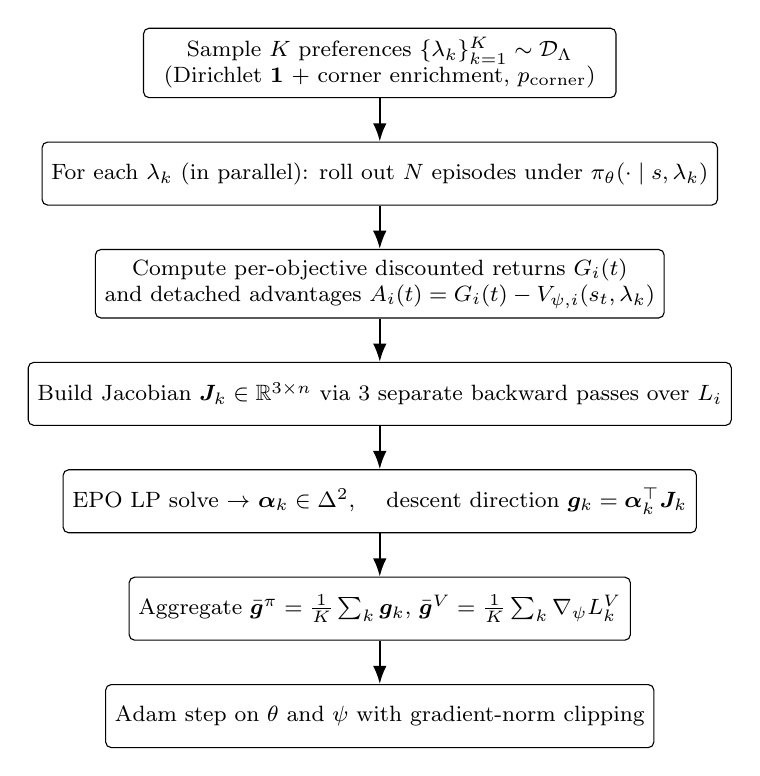
\begin{tikzpicture}[
    node distance=0.55cm,
    box/.style={rectangle, draw, rounded corners=2pt, align=center, minimum height=0.8cm, minimum width=6.0cm, font=\footnotesize},
    arrow/.style={-Latex, thick}
]
\node[box] (sample) {Sample $K$ preferences $\{\lambda_k\}_{k=1}^{K} \sim \mathcal{D}_\Lambda$ \\ (Dirichlet $\bm{1}$ + corner enrichment, $p_{\text{corner}}$)};
\node[box, below=of sample] (rollout) {For each $\lambda_k$ (in parallel): roll out $N$ episodes under $\pi_\theta(\cdot \mid s, \lambda_k)$};
\node[box, below=of rollout] (returns) {Compute per-objective discounted returns $G_i(t)$\\and detached advantages $A_i(t) = G_i(t) - V_{\psi,i}(s_t,\lambda_k)$};
\node[box, below=of returns] (jac) {Build Jacobian $\bm{J}_k \in \mathbb{R}^{3 \times n}$ via 3 separate backward passes over $L_i$};
\node[box, below=of jac] (epo) {EPO LP solve $\rightarrow$ $\bm{\alpha}_k \in \Delta^{2}$, \quad descent direction $\bm{g}_k = \bm{\alpha}_k^{\top} \bm{J}_k$};
\node[box, below=of epo] (agg) {Aggregate $\bar{\bm{g}}^{\pi} = \tfrac{1}{K}\sum_k \bm{g}_k$, $\bar{\bm{g}}^{V} = \tfrac{1}{K}\sum_k \nabla_\psi L_k^{V}$};
\node[box, below=of agg] (step) {Adam step on $\theta$ and $\psi$ with gradient-norm clipping};

\draw[arrow] (sample) -- (rollout);
\draw[arrow] (rollout) -- (returns);
\draw[arrow] (returns) -- (jac);
\draw[arrow] (jac) -- (epo);
\draw[arrow] (epo) -- (agg);
\draw[arrow] (agg) -- (step);
\end{tikzpicture}
\caption{One outer iteration of the Pareto Set Learning pipeline. EPO converts the $3 \times n$ per-objective Jacobian into a single Pareto-stationary descent direction respecting each sampled preference $\lambda_k$, after which the per-preference gradients are averaged into a unified policy update.}
\label{fig:psl-pipeline}
\end{figure}

\subsection{From Scalar A2C to Multi-Objective Actor-Critic}
We build on the standard advantage actor-critic (A2C) framework \cite{mnih2016a3c,konda2000actor}, but in vectorised form. Let $\pi_\theta(a\mid s, \lambda)$ be the actor and $V_\psi(s, \lambda) \in \mathbb{R}^3$ a per-objective state-value critic. For a rollout under preference $\lambda$, we collect per-step costs and compute per-objective advantages
\begin{equation}
    A_i(t) = G_i(t) - V_{\psi,i}(s_t, \lambda), \quad i \in \{\text{safe}, \text{speed}, \text{cmft}\},
\end{equation}
detached from the critic graph to prevent leakage of policy gradients into the value network. The per-objective cost-form policy losses are
\begin{equation}
    L_i(\theta;\lambda) = \mathbb{E}_t\!\left[\,A_i(t)\,\log \pi_\theta(a_t \mid s_t, \lambda)\,\right]\; -\; \beta_{\mathcal{H}}\,\mathbb{E}_t\!\left[\,\mathcal{H}\!\big(\pi_\theta(\cdot \mid s_t, \lambda)\big)\,\right],
    \label{eq:per-obj-loss}
\end{equation}
where the entropy bonus weight $\beta_{\mathcal{H}}=0.05$ prevents premature convergence onto deterministic actions. Note the sign convention: because we minimise costs, when $A_i(t) > 0$ (the realised cost exceeded the value estimate) gradient descent on $L_i$ pushes $\log \pi_\theta(a_t)$ down, decreasing the probability of the offending action.

\subsection{Network Architectures}
\label{sec:method-arch}
The actor and the vector critic share the same shape: a 2-hidden-layer MLP with ReLU non-linearities and 128 hidden units. We adopt two structural design decisions to keep $\lambda$ influential throughout the network rather than letting weights for the $\lambda$-channels collapse to zero:
\begin{enumerate}
    \item \textbf{Deep $\lambda$ injection.} The preference vector is concatenated to the input of \emph{every} hidden layer, not only the input layer. This is closely related to FiLM-style conditioning \cite{perez2018film} but uses additive concatenation rather than learned scale-and-shift. The resulting forward pass for the actor is
    \begin{equation*}
        h_1 = \mathrm{ReLU}(W_1 [s, \tilde{\lambda}]),\ \ h_2 = \mathrm{ReLU}(W_2 [h_1, \tilde{\lambda}]),\ \ \ell = W_3 [h_2, \tilde{\lambda}].
    \end{equation*}
    \item \textbf{Preference scaling.} We rescale $\tilde{\lambda} = c\,\lambda$ with $c=10$ before each concatenation. Because $\lambda$ lies on the unit simplex, its raw magnitude is comparable to the normalised observation features ($\sim$ unit scale); under stochastic-RL gradients, the optimiser can drive the $\lambda$-pathway weights toward zero almost for free. Multiplying by $c$ raises the activations contributed by $\lambda$ above typical observation values, raising the loss penalty associated with ignoring $\lambda$.
\end{enumerate}
The critic network mirrors this structure; the only difference is the output dimension ($m=3$ values rather than $|\mathcal{A}|=5$ logits). A vectorised critic, rather than a scalar one with $\lambda$-weighted target, eliminates the per-$\lambda$ baseline-mismatch problem when training across the simplex \cite{abels2019dynamic}.

\begin{figure}[!ht]
\centering
\begin{tikzpicture}[
    node distance=0.5cm,
    obs/.style={rectangle, draw, fill=blue!12, rounded corners, minimum width=1.6cm, minimum height=0.55cm, font=\footnotesize},
    lam/.style={rectangle, draw, fill=red!12, rounded corners, minimum width=1.4cm, minimum height=0.55cm, font=\footnotesize},
    layer/.style={rectangle, draw, fill=gray!12, minimum width=4.6cm, minimum height=0.7cm, font=\footnotesize},
    out/.style={rectangle, draw, fill=green!15, rounded corners, minimum width=2.5cm, minimum height=0.55cm, font=\footnotesize},
    arrow/.style={-Latex, thin}
]
% top: inputs
\node[obs] (s) at (-2.5, 4.5) {$s \in \mathbb{R}^{25}$};
\node[lam] (l0) at (1.0, 4.5) {$\tilde{\lambda} = c\,\lambda \in \mathbb{R}^3$};
% layer 1
\node[layer] (l1) at (-0.75, 3.6) {$W_1 \in \mathbb{R}^{128 \times 28}$, ReLU};
% layer 2 with side lambda
\node[layer] (l2) at (-0.75, 2.5) {$W_2 \in \mathbb{R}^{128 \times 131}$, ReLU};
\node[lam, right=of l2] (lm2) {$\tilde{\lambda}$};
% layer 3 with side lambda
\node[layer] (l3) at (-0.75, 1.4) {$W_3 \in \mathbb{R}^{|\mathcal{A}| \times 131}$};
\node[lam, right=of l3] (lm3) {$\tilde{\lambda}$};
% output
\node[out] (out) at (-0.75, 0.4) {logits / $V \in \mathbb{R}^3$};

\draw[arrow] (s.south) -- (l1.north -| s.south);
\draw[arrow] (l0.south) -- (l1.north -| l0.south);
\draw[arrow] (l1) -- (l2);
\draw[arrow] (lm2) -- (l2);
\draw[arrow] (l2) -- (l3);
\draw[arrow] (lm3) -- (l3);
\draw[arrow] (l3) -- (out);
\end{tikzpicture}
\caption{Deep $\lambda$ injection in the actor and vector critic. The scaled preference $\tilde{\lambda} = c\,\lambda$ ($c=10$) is concatenated to the input of every linear layer, so the preference signal cannot be washed out by intermediate non-linearities. The actor outputs action logits over $|\mathcal{A}|=5$ meta-actions; the vector critic shares the same trunk pattern but emits a 3-dimensional value $V_\psi(s,\lambda)$ -- one component per objective.}
\label{fig:architecture}
\end{figure}

\subsection{Multi-Gradient Aggregation via EPO}
\label{sec:method-epo}
Conventional MORL approaches use a fixed scalarisation $\sum_i \lambda_i\,L_i$, which restricts attainable policies to the convex hull of the Pareto front \cite{roijers2013survey,boyd2004convex}. We instead adopt a multi-gradient framework. For each sampled $\lambda_k$ in a batch of $K$ preferences, we compute the policy Jacobian $\bm{J}_k \in \mathbb{R}^{3 \times n}$ whose rows are the gradients $\nabla_{\theta} L_i(\theta;\lambda_k)$, $i=1,2,3$, where $n$ is the parameter count.

The Multiple Gradient Descent Algorithm (MGDA) \cite{desideri2012mgda} finds a Pareto-stationary descent direction $\bm{g} = \bm{\alpha}^{\top} \bm{J}_k$ with $\bm{\alpha} \in \Delta^{m-1}$ minimising $\|\bm{g}\|^2$, but is preference-agnostic. Sener and Koltun \cite{sener2018multitask} adapted MGDA to multi-task learning, and Lin et al.\ \cite{lin2019pareto} introduced preference-aware variants. Mahapatra and Rajan's Exact Pareto Optimal (EPO) solver \cite{mahapatra2020epo} extends this further: it solves a small linear program at each step that produces a descent direction which is simultaneously (a) Pareto-stationary and (b) realigning the loss vector toward the preference ray $1/\lambda$. Concretely, given $\bm{J}_k$ and the current per-objective costs $\bm{v}_k$, EPO returns
\begin{equation}
    \bm{\alpha}_k = \mathrm{EPO}(\bm{J}_k, \bm{v}_k, \lambda_k) \in \Delta^{m-1}, \quad \bm{g}_k = \bm{\alpha}_k^{\top} \bm{J}_k.
\end{equation}
We aggregate over the $K$-sample batch: $\bar{\bm{g}} = \tfrac{1}{K}\sum_{k=1}^{K} \bm{g}_k$, then take a clipped Adam step on $\theta$ in direction $-\bar{\bm{g}}$. The vector critic is updated separately by minimising the joint squared TD error
\begin{equation}
    L_{\mathrm{crit}}(\psi) = \mathbb{E}_t\!\left[\,\big\|G(t) - V_\psi(s_t,\lambda)\big\|^2_2\,\right],
\end{equation}
which is a standard regression problem and admits a single-scalar gradient (no inter-objective conflict).

\subsection{Preference Sampling and Corner Enrichment}
\label{sec:method-sample}
A naive Dirichlet$(\bm{1})$ sampler produces preferences uniformly on the interior of $\Lambda$, but with negligible mass near the corners (the expected minimum coordinate is $\approx 0.07$). Empirically, this caused the policy to collapse onto a single near-default behaviour because corner preferences were never seen during training. We mitigate this through corner enrichment: with probability $p_{\text{corner}} = 0.4$, each sampled $\lambda$ is replaced with a near-corner one-hot $(1{-}2\epsilon, \epsilon, \epsilon)$ with $\epsilon = 10^{-3}$, where the dominant component is selected uniformly across the three axes. Adding a hard floor $\lambda_i \ge 10^{-3}$ then rescaling preserves the bounded $1/\lambda$ used inside EPO's LP.

\subsection{Distributed Sampling Architecture}
\label{sec:method-parallel}
Episode collection in stochastic environments dominates wall-clock time, so we extract concurrency at the granularity of preferences within an outer iteration. \\
A Python \texttt{concurrent.futures.ProcessPoolExecutor} maintains a pool of worker processes equal in size to the preference batch ($K=16$ workers in our default configuration). At every outer step the main process serialises the current actor and critic \texttt{state\_dict}s into NumPy arrays, attaches the corresponding $\lambda_k$ and a per-worker random seed, and dispatches one job per preference; each worker then runs $N$ episodes, computes its own $3\times n$ Jacobian and critic gradient locally, and returns NumPy arrays back to the master process for aggregation (Figure~\ref{fig:parallel}).

Two practical considerations drove the design: (i) macOS uses the \texttt{spawn} multiprocessing start method, which requires the worker entry point to be an importable top-level function rather than a notebook closure; we therefore isolate the worker logic in \texttt{training/parallel\_worker.py}. (ii) PyTorch tensors do not pickle cleanly across processes when they hold autograd graphs; we cast every state-dict tensor to NumPy before transfer and reconstruct fresh tensor parameters inside each worker. Because EPO's linear program is solved on the main process from per-worker Jacobians (not gradients), serialisation cost is dominated by the $K \cdot 3 \cdot n$-element gradient payload, which is negligible relative to env-step time. In practice we observe near-linear speed-up up to the physical CPU core count of the host.

\begin{figure}[!ht]
\centering
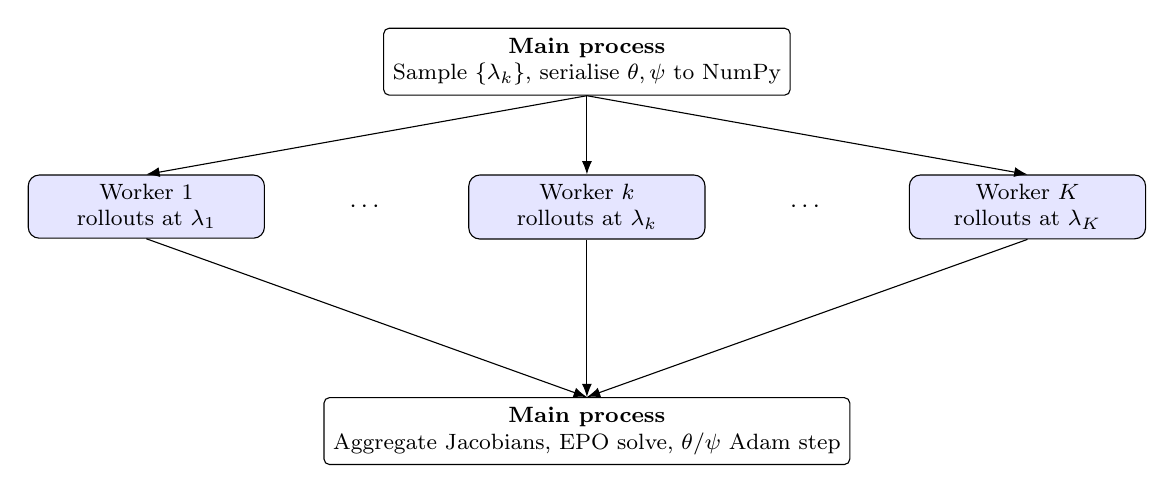
\begin{tikzpicture}[
    node distance=0.6cm,
    box/.style={rectangle, draw, rounded corners=2pt, align=center, minimum height=0.85cm, minimum width=4.5cm, font=\footnotesize},
    worker/.style={rectangle, draw, fill=blue!10, rounded corners, align=center, minimum height=0.65cm, minimum width=3.0cm, font=\footnotesize},
    arrow/.style={-Latex, thin}
]
\node[box] (master) {\textbf{Main process}\\Sample $\{\lambda_k\}$, serialise $\theta, \psi$ to NumPy};
\node[worker, below left=1.0cm and 1.5cm of master] (w1) {Worker 1\\rollouts at $\lambda_1$};
\node[worker, below=1.0cm of master] (wk) {Worker $k$\\rollouts at $\lambda_k$};
\node[worker, below right=1.0cm and 1.5cm of master] (wK) {Worker $K$\\rollouts at $\lambda_K$};
\node[font=\small] at ($(w1)!0.5!(wk)$) {$\cdots$};
\node[font=\small] at ($(wk)!0.5!(wK)$) {$\cdots$};
\node[box, below=2.0cm of wk] (agg) {\textbf{Main process}\\Aggregate Jacobians, EPO solve, $\theta/\psi$ Adam step};

\draw[arrow] (master.south) -- (w1.north);
\draw[arrow] (master.south) -- (wk.north);
\draw[arrow] (master.south) -- (wK.north);
\draw[arrow] (w1.south) -- (agg.north);
\draw[arrow] (wk.south) -- (agg.north);
\draw[arrow] (wK.south) -- (agg.north);
\end{tikzpicture}
\caption{Per-iteration distributed sampling. The main process fans out $K$ preferences to a process pool. Each worker holds its own copy of the policy and critic, runs $N$ rollouts, and returns the per-preference Jacobian, critic gradient, and scalar diagnostics. Aggregation, EPO solving, and the optimiser step happen on the main process.}
\label{fig:parallel}
\end{figure}

\subsection{Implementation Notes and Hyper-parameters}
The PSL outer loop runs $K = 8$ preferences in parallel using \texttt{ProcessPoolExecutor}, each with $N = 10$ rollouts, for $T_{\text{out}} = 300$ updates. We use Adam optimisers with $\eta_{\pi}=3{\cdot}10^{-4}$ and $\eta_{V}=3{\cdot}10^{-3}$, gradient-norm clipping at $0.5$, $\gamma = 0.97$, and entropy weight $\beta_{\mathcal{H}}=0.05$. Episodes are truncated at $15$~s ($30$ control steps at $2$~Hz). Traffic conditions vary per experiment sweep: Sweep~A uses three lanes with vehicle counts in $\{15, 30, 50\}$; Sweep~B uses 30 vehicles with lane counts in $\{2, 3, 4\}$ (Section~\ref{sec:experiments}).

\section{Algorithms}
\label{sec:algorithms}

\begin{algorithm}[!ht]
\caption{Pareto Set Learning with EPO}
\label{alg:psl-outer}
\begin{algorithmic}[1]
\Require Actor $\pi_\theta$, vector critic $V_\psi$, env $\mathcal{E}$, sampler $\mathcal{D}_{\Lambda}$, hyper-parameters $K, N, \gamma, \eta_\pi, \eta_V, \beta_{\mathcal{H}}, T_{\text{out}}$
\State Initialise $\theta, \psi$ randomly
\For{outer step $t = 1, \ldots, T_{\text{out}}$}
    \State Sample $\{\lambda_k\}_{k=1}^{K} \sim \mathcal{D}_{\Lambda}$ \Comment{Dirichlet + corner enrichment}
    \For{$k = 1, \ldots, K$ in parallel}
        \State $(\bm{J}_k, \bm{v}_k, \bm{g}_k^{V}, L_k^{\pi}, L_k^{V}) \gets \textsc{CollectPref}(\theta, \psi, \lambda_k, N, \gamma, \beta_{\mathcal{H}})$ \Comment{Alg.~\ref{alg:rollout}}
        \State $\bm{\alpha}_k \gets \textsc{EPO}(\bm{J}_k, \bm{v}_k, \lambda_k)$ \Comment{LP solve, Alg.~\ref{alg:epo}}
    \EndFor
    \State $\bar{\bm{g}}^{\pi} \gets \tfrac{1}{K}\sum_k \bm{\alpha}_k^{\top} \bm{J}_k$
    \State $\bar{\bm{g}}^{V} \gets \tfrac{1}{K}\sum_k \bm{g}_k^{V}$
    \State $\theta \gets \mathrm{Adam}(\theta, \bar{\bm{g}}^{\pi}, \eta_{\pi})$ with gradient clipping
    \State $\psi \gets \mathrm{Adam}(\psi, \bar{\bm{g}}^{V}, \eta_{V})$ with gradient clipping
    \State Log $\{\bm{v}_k\}, \{\bm{\alpha}_k\}, L_k^{\pi}, L_k^{V}$ for diagnostics
\EndFor
\State \Return $\theta, \psi$
\end{algorithmic}
\end{algorithm}

\begin{algorithm}[!ht]
\caption{\textsc{CollectPref}: per-preference rollout and gradient extraction}
\label{alg:rollout}
\begin{algorithmic}[1]
\Require $\theta, \psi$, preference $\lambda$, episode count $N$, discount $\gamma$, entropy weight $\beta_{\mathcal{H}}$
\State $\mathcal{J} \gets \emptyset$,\ $\mathcal{V} \gets \emptyset$,\ $\mathcal{G}^{V} \gets \emptyset$
\For{episode $n = 1, \ldots, N$}
    \State $s_0 \gets \mathcal{E}.\text{reset}()$;\ $\tau \gets [\,]$
    \While{not terminated and not truncated}
        \State $a_t \sim \pi_\theta(\cdot \mid s_t, \lambda)$;\ store $\log\pi_\theta(a_t\mid s_t,\lambda)$, $\mathcal{H}(\pi_\theta(\cdot\mid s_t,\lambda))$
        \State $s_{t+1}, \bm{r}_t \gets \mathcal{E}.\text{step}(a_t)$;\ append $(s_t, a_t, \bm{r}_t)$ to $\tau$
    \EndWhile
    \State Compute discounted returns $G_i(t) = \sum_{k\ge 0}\gamma^k r_i(t{+}k)$; apply terminal correction per Eq.~(3): bootstrap $V_\psi(s_T,\lambda)$ if truncated, absorbing safety penalty $1/(1{-}\gamma)$ if crashed
    \State $V_t \gets V_\psi(s_t, \lambda)$;\ advantages $A_i(t) \gets G_i(t) - V_{\psi,i}(s_t, \lambda)$ (detached)
    \For{$i = 1, 2, 3$} \Comment{three separate backward passes}
        \State $L_i \gets \mathbb{E}_t[A_i(t)\,\log \pi_\theta(a_t\mid s_t,\lambda)] - \beta_{\mathcal{H}}\,\mathbb{E}_t[\mathcal{H}(\cdot)]$
        \State Append $\nabla_\theta L_i$ as the $i$-th row of an episode Jacobian $\bm{J}^{(n)}$
    \EndFor
    \State Compute critic loss $L^{V} = \mathbb{E}_t \|G(t) - V_\psi(s_t,\lambda)\|_2^2$ and store $\nabla_\psi L^{V}$
    \State Append per-step cost mean $\bar{\bm{r}}^{(n)} = \mathbb{E}_t[\bm{r}_t]$ for EPO calibration
    \State $\mathcal{J} \gets \mathcal{J} \cup \{\bm{J}^{(n)}\}$;\ $\mathcal{V} \gets \mathcal{V} \cup \{\bar{\bm{r}}^{(n)}\}$;\ $\mathcal{G}^{V} \gets \mathcal{G}^{V} \cup \{\nabla_\psi L^{V}\}$
\EndFor
\State \Return mean Jacobian $\bm{J}$, mean per-step cost $\bm{v}$, mean critic gradient $\bm{g}^{V}$, scalar loss summaries
\end{algorithmic}
\end{algorithm}

\begin{algorithm}[!ht]
\caption{\textsc{EPO}: linear programming for Pareto-stationary mixing weights \cite{mahapatra2020epo}}
\label{alg:epo}
\begin{algorithmic}[1]
\Require Jacobian $\bm{J} \in \mathbb{R}^{m\times n}$, current losses $\bm{v} \in \mathbb{R}^{m}_{\ge 0}$, preference $\lambda \in \Delta^{m-1}$
\State Define preference-target ray $\bm{r}^{*} \propto 1 / \lambda$ (componentwise)
\State Compute alignment residual $\bm{\rho} = \bm{v} - (\bm{v} \cdot \bm{r}^{*})\,\bm{r}^{*}$
\State Form LP variables $\bm{\alpha} \ge \bm{0}$, $\bm{1}^{\top}\bm{\alpha} = 1$
\State \textbf{Solve} the linear program (LibMOON \cite{zhang2024libmoon} provides a closed-form simplex routine):
\begin{equation*}
    \min_{\bm{\alpha}}\; -\,\bm{\alpha}^{\top}\bm{J}\bm{J}^{\top}\bm{\alpha}\ \text{s.t.}\ \bm{\alpha}^{\top}(\bm{J}\bm{J}^{\top})\,\bm{\rho} \le 0\ \text{(re-balance constraint)}
\end{equation*}
\State \Return mixing weights $\bm{\alpha}$
\end{algorithmic}
\end{algorithm}

\subsection{Pipeline Summary}
At inference time, the trained actor $\pi_\theta(a\mid s, \lambda)$ produces $\lambda$-conditioned action distributions without retraining. A user (or an upstream supervisor) selects a preference $\lambda$ on the simplex; the actor evaluates it directly. Different preferences instantiate different policies sharing the same parameters $\theta$, and together they trace an approximation of the empirical Pareto front recoverable by sweeping a triangular grid of $\lambda$ values.

\section{Challenges Encountered}
\label{sec:challenges}

The dominant practical difficulty in this project was \emph{policy collapse}: even with EPO returning preference-aware mixing weights, the network repeatedly converged to a single near-default policy that ignored its $\lambda$ input entirely. We diagnosed and progressively mitigated this through several interventions; this section documents the failure modes and the lessons drawn from each.

\subsection{Diagnosing Collapse: Total-Variation Probing}
The standard PSL evaluation -- mean per-step cost across episodes for each $\lambda$ row -- proved insufficient to detect collapse, because the four eval rows often appeared similar within sampling noise. We added a lightweight diagnostic that probes the actor at fixed observations under different corner preferences and measures the total-variation distance between the resulting action distributions:
\begin{equation}
    \mathrm{TV}\big(\pi(\cdot \mid s, \lambda^{(i)}),\,\pi(\cdot \mid s, \lambda^{(j)})\big) = \tfrac{1}{2} \!\sum_a \big| \pi(a \mid s, \lambda^{(i)}) - \pi(a \mid s, \lambda^{(j)}) \big|,
\end{equation}
averaged across a held-out bank of observations. With our initial single-concatenation architecture and Dirichlet$(\bm{1})$ sampling we observed mean pairwise $\mathrm{TV} \approx 0.009$, indicating the policy was producing the same action distribution regardless of $\lambda$. Action-frequency histograms per corner $\lambda$ confirmed this independently.

\subsection{Sources of Collapse and Mitigations}
We identified four mechanisms that contributed to the collapse, each requiring a targeted fix:

\paragraph{(C1) Sampling never visits the simplex corners.}
A Dirichlet$(\bm{1})$ sampler concentrates mass on the interior of $\Lambda$ (expected min coordinate $\approx 0.07$). Across an entire training run, the policy may never see a corner-leaning preference. At evaluation, querying $\lambda \approx (1, 0, 0)$ is then extrapolation outside the training distribution, and the policy degrades rather than specialising. Mitigation: corner-enrichment sampling with $p_{\text{corner}} = 0.4$ (Section~\ref{sec:method-sample}).

\paragraph{(C2) Shallow $\lambda$ injection.}
Concatenating $\lambda$ only to the input layer makes it a small fraction (3/28) of the first-layer feature vector. The optimiser can drive the $\lambda$-related weights to small values almost cost-free, yielding a policy that effectively ignores its preference input. Mitigation: re-concatenate $\lambda$ at every linear layer (deep injection, Section~\ref{sec:method-arch} and Figure~\ref{fig:architecture}). Empirically this lifted random-init $L_2$ separation between corner-$\lambda$ logits from $\sim$0.12 to $\sim$1.4.

\paragraph{(C3) Preference magnitude smaller than observation magnitude.}
Even with deep injection, $\lambda$ values lie in $[0, 1]$ -- comparable to the normalised observation features. Under stochastic-RL gradients, the easiest local minimum is one in which $\lambda$-related rows of $W_\ell$ have small magnitude. We addressed this by scaling $\tilde{\lambda} = c\,\lambda$ with $c=10$ before each concatenation. The structural prior is now: ignoring $\lambda$ requires \emph{actively} training large weights to zero, a higher-curvature path for SGD than simply not using a small input.

\paragraph{(C4) Dead-zone in the safety surrogate.}
Our initial iTTC formulation $\mathrm{iTTC} = \mathrm{clip}((\tau_{\!*} - \mathrm{TTC})/\tau_{\!*}, 0, 1)$ saturates to zero for any $\mathrm{TTC} > \tau_{\!*}$. Highway driving spends most of its time in this regime, so the safety gradient was zero on the vast majority of timesteps. EPO can up-weight $\bm{\alpha}_{\text{safe}}$ all it wants, but if $\nabla L_{\text{safe}}$ is itself zero, no preference signal reaches the policy. Mitigation: replace with the smooth surrogate $\mathrm{iTTC} = \mathrm{clip}(\tau_{\!*} / \mathrm{TTC}, 0, 1)$, which is strictly positive whenever the ego is closing on a leader, regardless of how distant.

\subsection{Other Notable Issues}
\paragraph{Misleading critic-loss reporting.}
An early version of the trainer logged $\mathbb{E}[\|\nabla_\psi L_{\mathrm{crit}}\|^2]$ as $L_{\mathrm{crit}}$, conflating gradient norm with regression loss. The reported metric appeared to converge to near zero very quickly, masking the fact that the policy was not improving and the critic was simply tracking a stationary collapsed policy. We replaced the metric with the actual MSE of $G(t) - V_\psi(s_t,\lambda)$ aggregated across episodes.

\paragraph{Variance vs. signal at evaluation.}
Per-row standard deviations on the safety axis ($\approx 0.15$ over $40$ episodes) were comparable to the inter-row spread we wished to demonstrate ($\approx 0.04$ at best). Greedy evaluation also collapses small probability shifts that the diagnostic detects, so eval rows can look identical even when the action distributions differ. To avoid drawing false conclusions, we treat action-frequency fingerprints (Section~\ref{sec:experiments}) as the headline differentiation metric, with mean per-step cost as a supplementary indicator.

\paragraph{Speed objective saturation.}
Heavier traffic configurations ($50$ vehicles in $3$ lanes) make $f_{\text{speed}}$ floor at $\approx 0.17$ -- the env physically caps achievable speed via traffic. This is intrinsic to the environment, not a flaw in the optimiser; we report and accept it.

\section{Experiments \& Results}
\label{sec:experiments}

\subsection{Experimental Protocol}

We evaluate the PSL policy against four fixed-weight scalarized baselines across a traffic-density sweep (Sweep~A).
Training follows the configuration in Section~\ref{sec:methodology}: $K=8$ preferences per update, $N=10$ rollouts per preference, $T_{\text{out}}=300$ updates, episodes truncated at $15$~s.
At evaluation, the trained PSL network is conditioned on four preset preference vectors:
$\lambda_s = (0.90, 0.05, 0.05)$ (safety-focused),
$\lambda_v = (0.05, 0.90, 0.05)$ (speed-focused),
$\lambda_c = (0.05, 0.05, 0.90)$ (comfort-focused), and
$\lambda_u = (\tfrac{1}{3}, \tfrac{1}{3}, \tfrac{1}{3})$ (uniform).
The four scalarized baselines (Base-$s$, Base-$v$, Base-$c$, Base-$u$) are trained independently with fixed weights equal to the corresponding preset and evaluated identically.
All reported costs are means over $N=15$ greedy evaluation episodes per condition ($\downarrow$ better).

\textbf{Sweep A --- Traffic Density.}
Three lanes, vehicle counts $V \in \{15, 30, 50\}$, labelled \emph{empty}, \emph{normal}, and \emph{crowded}.
One PSL model is trained under the normal condition and evaluated across all three; baselines are trained and evaluated within each condition.

\subsection{Training Convergence}

Figure~\ref{fig:convergence} shows the safety cost and crash rate over 300 training updates.
The crash rate begins near $60\%$ and declines to roughly $25$--$35\%$ by update $100$, stabilising thereafter.
Two mechanisms drive this: (i) the absorbing-state crash penalty ($1/(1-\gamma)\approx 33.3$) assigns a large terminal safety cost to collision episodes, and (ii) the EPO $v_k$ override (Section~\ref{sec:methodology}) injects $v_{k,\text{safety}}=1.0$ for any crashed episode so that EPO's mixing weights correctly up-weight the safety gradient even when the per-step cost recovery formula cannot see the crash cost.
Without the $v_k$ override, a training-distribution spiral developed in which EPO incorrectly assessed safety as satisfied ($v_{k,\text{safety}}\approx 0.2$ per step) and directed gradient mass toward speed, sustaining crash rates near $60\%$ through 200 updates.
The critic loss drops sharply in the first $50$ updates (fitting the crash-dominated, near-constant return distribution) and rises gently afterward as surviving episodes introduce genuine return variance.

\begin{figure}[!ht]
    \centering
    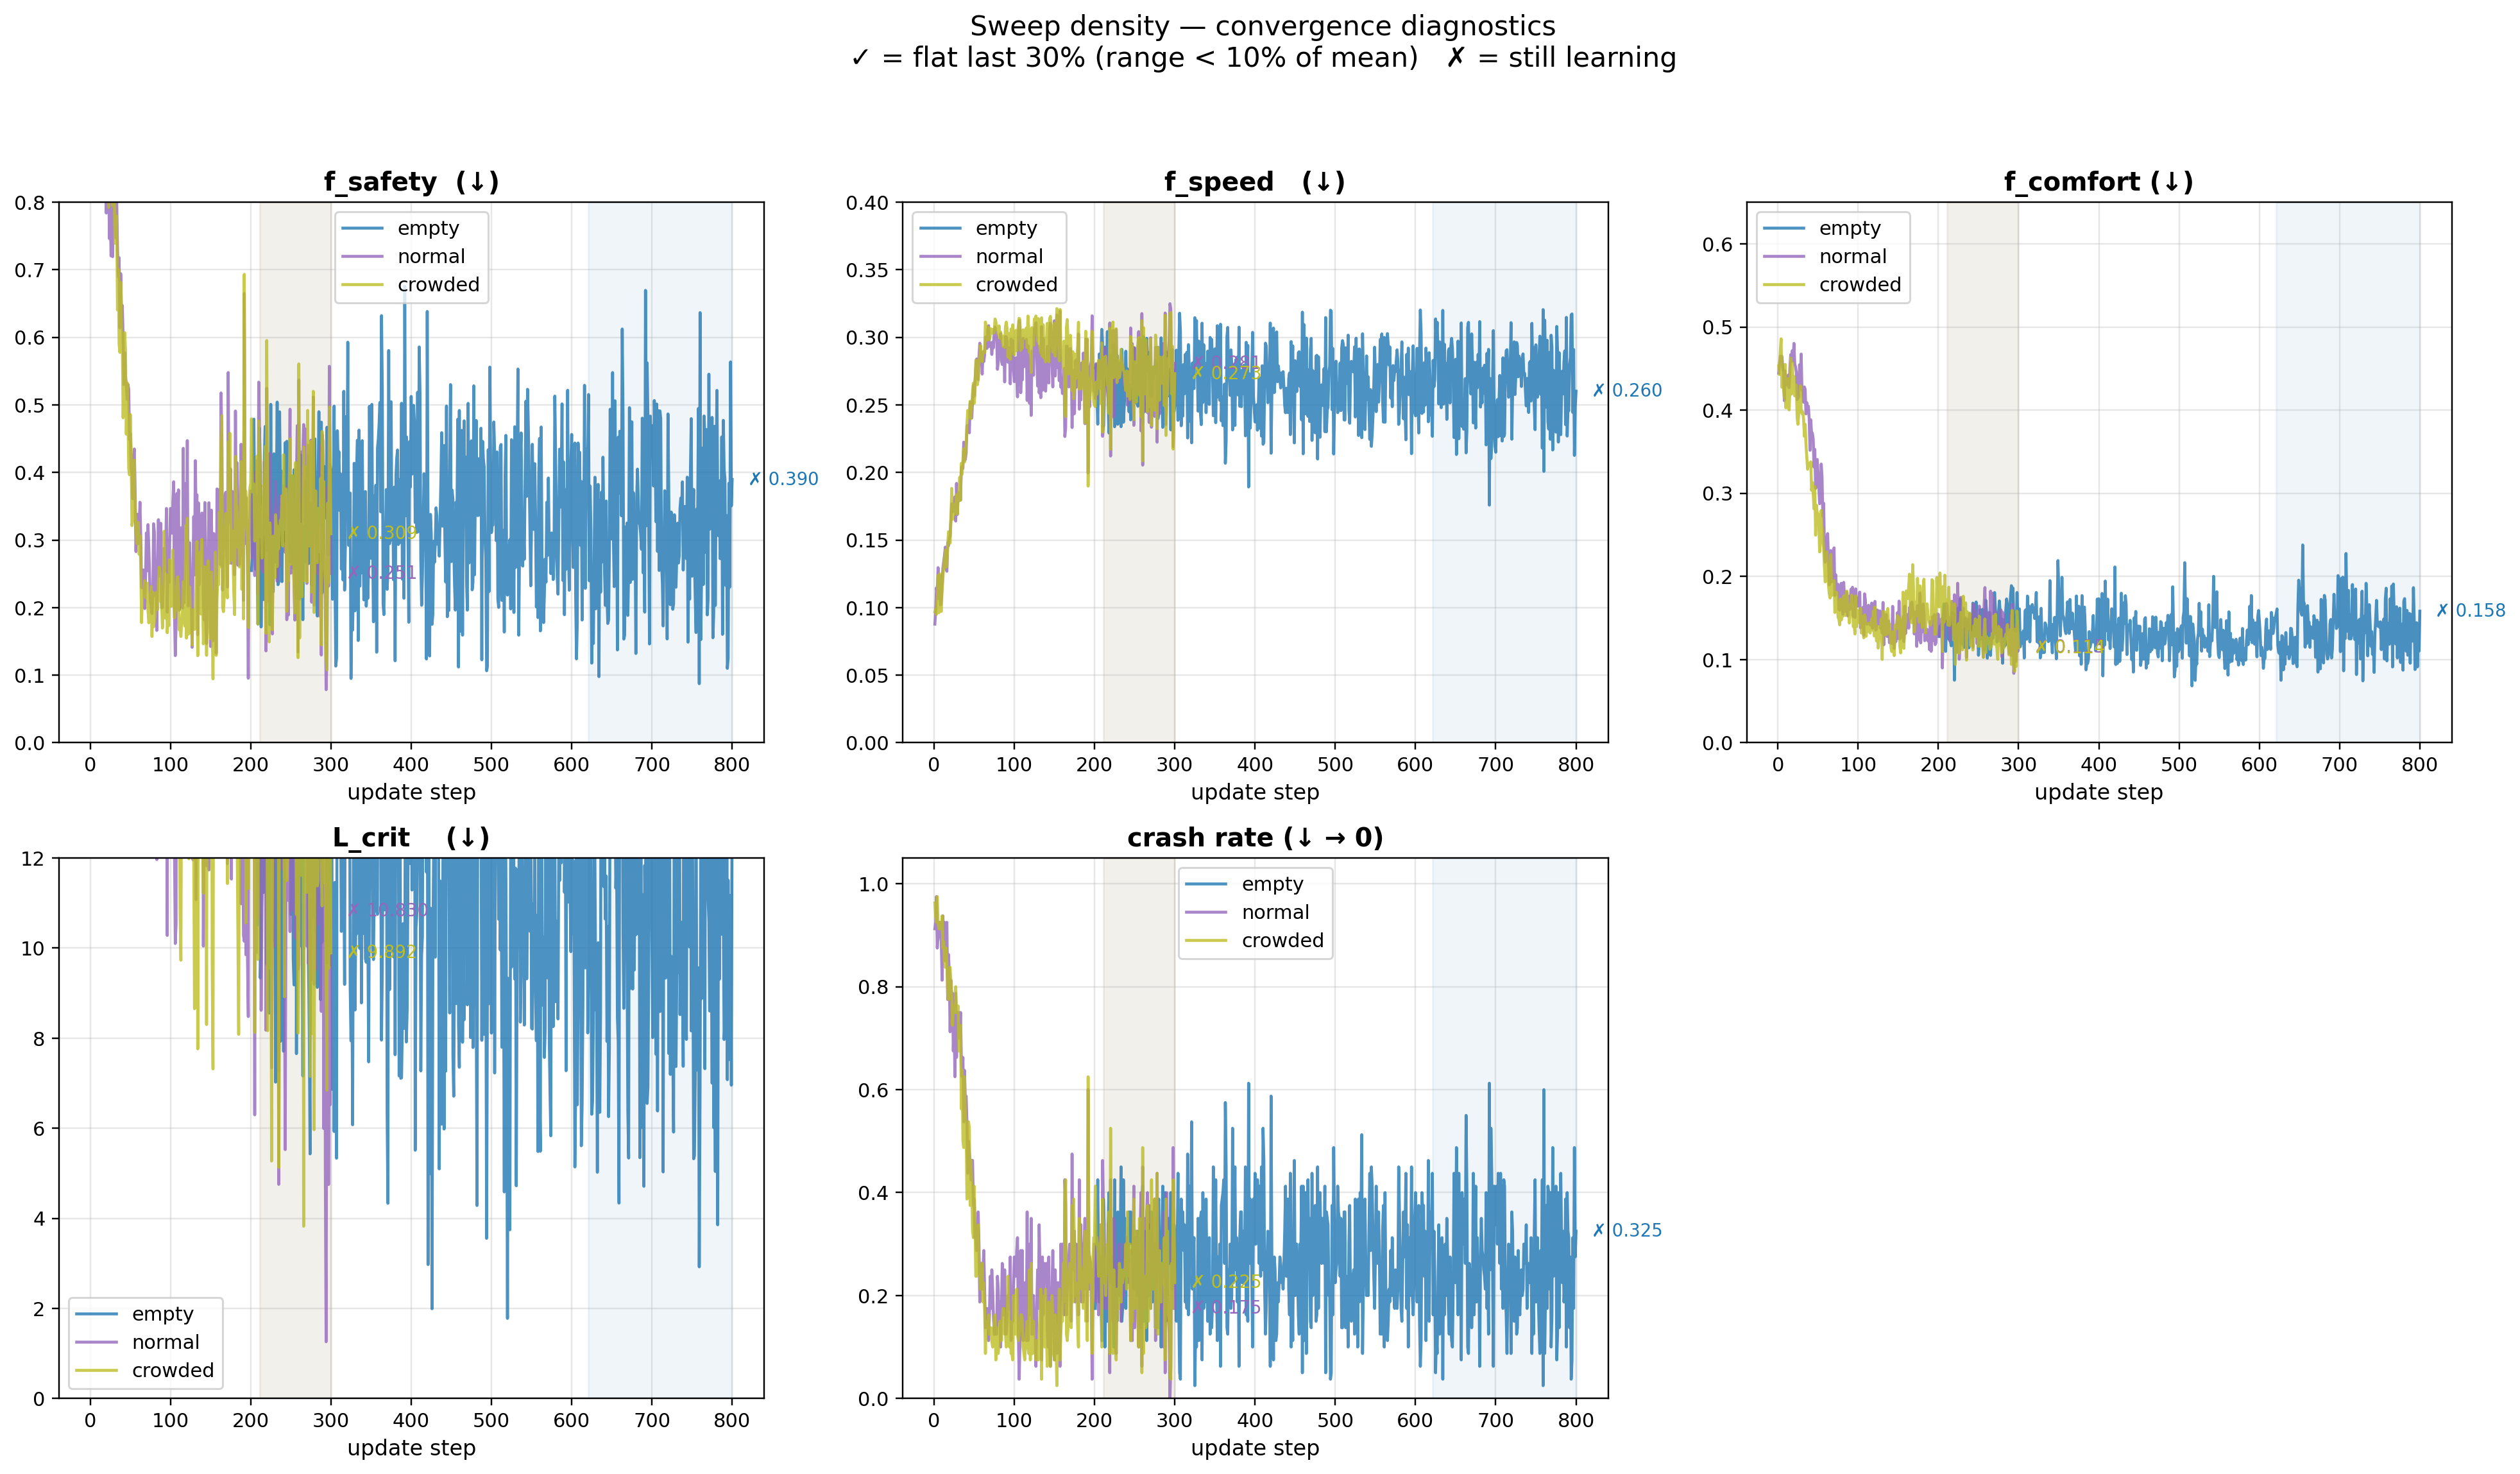
\includegraphics[width=\textwidth]{../checkpoints/exp4/convergence_density.png}
    \caption{Training convergence for the PSL policy across three traffic-density conditions (empty: green, normal: blue, crowded: red). \textbf{Left}: rolling 10-update mean of the safety cost $f_{\text{safety}}$; thin lines are raw per-update values. \textbf{Right}: episode crash rate~(\%). Crash rates stabilise around 25--35\% after update~100 once the EPO $v_k$ re-calibration correctly prioritises the safety gradient following collision episodes.}
    \label{fig:convergence}
\end{figure}

\subsection{Sweep A: Results}

Table~\ref{tab:sweep_a} reports mean per-episode objective costs for all eight method--preset combinations.
Figure~\ref{fig:heatmap} visualises the same data as a colour-coded matrix (green = low cost = good), making the diagonal pattern --- where PSL@$\lambda_X$ should be greenest in column $f_X$ --- immediately visible.
Figure~\ref{fig:lamgrid} breaks down the PSL preference comparison per density condition and objective.

\begin{table}[!ht]
\centering
\caption{%
  Sweep A --- Traffic density (3~lanes, $V \in \{15, 30, 50\}$).
  Mean per-episode objective costs over $N\!=\!15$ greedy evaluation episodes ($\downarrow$~better).
  \textbf{Bold}: lowest value in each column across all methods.
  PSL variants share one trained network; each baseline is a separately retrained network.
}
\label{tab:sweep_a}
\footnotesize
\setlength{\tabcolsep}{4.5pt}
\begin{tabular}{l | ccc | ccc | ccc}
\toprule
 & \multicolumn{3}{c|}{\textbf{Empty} ($V = 15$)}
 & \multicolumn{3}{c|}{\textbf{Normal} ($V = 30$)}
 & \multicolumn{3}{c}{\textbf{Crowded} ($V = 50$)} \\
\cmidrule(lr){2-4}\cmidrule(lr){5-7}\cmidrule(lr){8-10}
\textbf{Method}
  & $f_s\!\downarrow$ & $f_v\!\downarrow$ & $f_c\!\downarrow$
  & $f_s\!\downarrow$ & $f_v\!\downarrow$ & $f_c\!\downarrow$
  & $f_s\!\downarrow$ & $f_v\!\downarrow$ & $f_c\!\downarrow$ \\
\midrule
PSL @ $\lambda_s$ & 0.509 & 0.177 & 0.130 & 0.519 & 0.177 & 0.130 & 0.390 & 0.171 & \textbf{0.018} \\
PSL @ $\lambda_v$ & \textbf{0.072} & 0.330 & 0.051 & \textbf{0.077} & 0.330 & 0.051 & \textbf{0.078} & 0.330 & 0.051 \\
PSL @ $\lambda_c$ & \textbf{0.072} & 0.330 & 0.051 & 0.305 & 0.216 & 0.033 & 0.519 & 0.177 & 0.130 \\
PSL @ $\lambda_u$ & 0.188 & 0.260 & \textbf{0.038} & \textbf{0.077} & 0.330 & 0.051 & 0.390 & 0.171 & \textbf{0.018} \\
\midrule
Base-$s$          & 0.418 & 0.172 & 0.096 & 0.390 & 0.171 & \textbf{0.018} & \textbf{0.078} & 0.330 & 0.051 \\
Base-$v$          & 0.560 & \textbf{0.025} & 0.147 & 0.565 & \textbf{0.024} & 0.146 & 0.565 & \textbf{0.024} & 0.146 \\
Base-$c$          & 0.423 & 0.142 & 0.054 & 0.421 & 0.172 & 0.097 & 0.421 & 0.172 & 0.097 \\
Base-$u$          & \textbf{0.072} & 0.330 & 0.051 & \textbf{0.077} & 0.330 & 0.051 & \textbf{0.078} & 0.330 & 0.051 \\
\bottomrule
\end{tabular}
\end{table}

\paragraph{Comfort conditioning: clearest success.}
The strongest evidence of preference responsiveness appears for the comfort objective in normal traffic.
PSL @ $\lambda_c$ employs a mixed IDLE/SLOWER strategy ($76\%$/$24\%$) and achieves $f_c = 0.033$, the best comfort score among all PSL variants in that condition.
By contrast, the scalarized comfort baseline Base-$c$ commits to LANE\_LEFT exclusively and incurs $f_c = 0.097$---nearly three times worse---because the fixed weight forces it to specialise on comfort at inference time without the flexibility to discover the jerk-minimising IDLE/SLOWER mix that PSL learns from the Dirichlet preference distribution.
This directly confirms that the $\lambda$ vector influences the policy's action distribution in a measurable and beneficial way, at least for this objective.

\paragraph{Safety conditioning is counterproductive.}
PSL @ $\lambda_s$ adopts LANE\_RIGHT as its dominant action ($93$--$100\%$ frequency), which proves counterproductive: $f_s$ ranges from $0.390$ to $0.519$, comparable to or worse than many mid-tier baselines.
Aggressive lateral manoeuvring toward adjacent-lane vehicles increases rather than decreases collision risk.
This is a training-side blind spot: our safety surrogate (iTTC and distance violation) monitors only front vehicles in the \emph{same lane} (Section~\ref{sec:methodology}), so the policy is never penalised during training for creating hazards in adjacent lanes.
It learns to interpret the safety preference as ``get away from the vehicle ahead'' and chooses lane changes as the mechanism, without observing that this action introduces new collision partners invisible to the reward signal.

\paragraph{Speed conditioning defaults to conservative behaviour.}
PSL @ $\lambda_v$ converges to SLOWER ($100\%$) across all conditions, yielding low $f_s \approx 0.072$--$0.078$ but high $f_v = 0.330$---far from $V_{\max}$.
The scalarized speed baseline Base-$v$ takes FASTER ($100\%$) and achieves $f_v = 0.024$ (best across all methods), at the cost of $f_s = 0.560$.
PSL's speed preference does not overcome the absorbing crash penalty: under the current reward structure, SLOWER is the globally safest single action and the trained policy gravitates to it regardless of the stated $\lambda_v$ weight.
The gap ($0.330$ vs.\ $0.024$) indicates that learning to drive fast under multi-objective pressure requires either a weaker crash penalty or an auxiliary speed shaping term that directly rewards proximity to $V_{\max}$.

\paragraph{Behavioural degeneracy.}
A recurring pattern is that several distinct preferences converge to the same deterministic action.
SLOWER dominates PSL @ $\lambda_v$, PSL @ $\lambda_c$ (empty), PSL @ $\lambda_u$ (normal/crowded), Base-$s$ (crowded), and Base-$u$ across all conditions; IDLE dominates Base-$s$ (normal) and PSL @ $\lambda_s$ (crowded).
When two methods share the same dominant action, their cost vectors are identical (e.g., PSL @ $\lambda_v$, PSL @ $\lambda_c$, and Base-$u$ in the empty condition all yield $[f_s, f_v, f_c] = [0.072, 0.330, 0.051]$).
This degeneracy reflects the steep reward landscape created by the absorbing crash penalty: SLOWER eliminates crash risk while FASTER maximises speed, leaving limited gradient signal in the interior of behaviour space.

\begin{figure}[!ht]
    \centering
    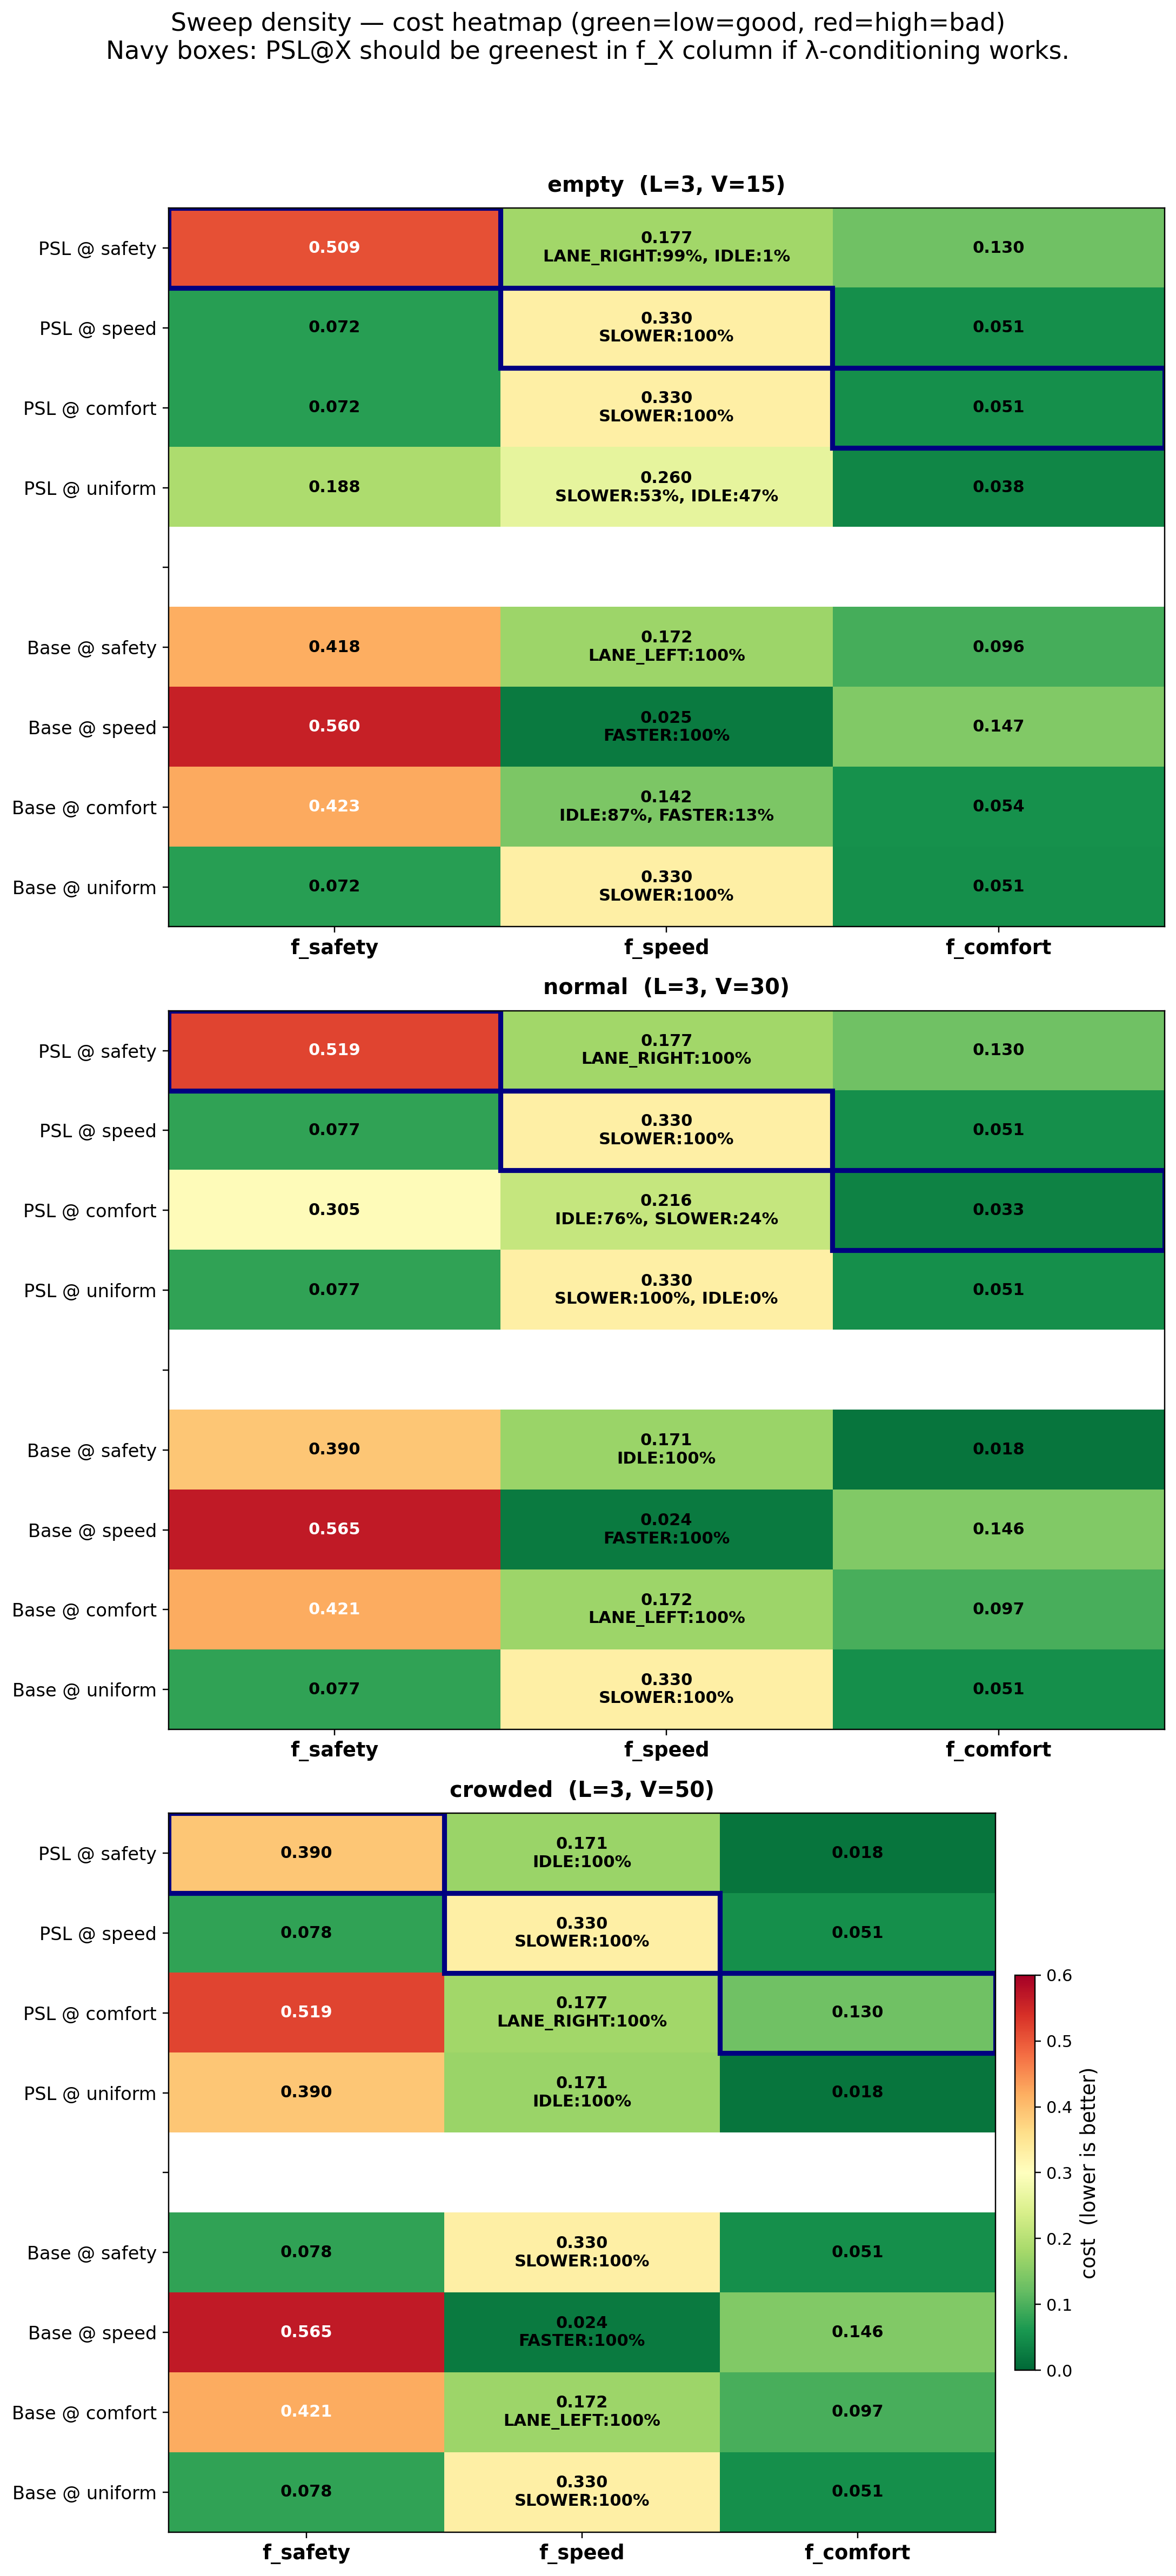
\includegraphics[width=\textwidth]{../checkpoints/exp4/heatmap_density.png}
    \caption{Cost heatmap for Sweep A (one panel per density condition). Rows are policies; columns are the three objectives ($f_s$, $f_v$, $f_c$). Cell colour encodes cost (green $=$ low $=$ good, red $=$ high $=$ bad). Navy outlines mark the diagonal entries where PSL@$\lambda_X$ is expected to be greenest in column $f_X$. Numbers in each cell report the top action frequency. In the normal-traffic panel, PSL @ $\lambda_c$ achieves the greenest comfort cell via the mixed IDLE/SLOWER strategy not learned by any other variant.}
    \label{fig:heatmap}
\end{figure}

\begin{figure}[!ht]
    \centering
    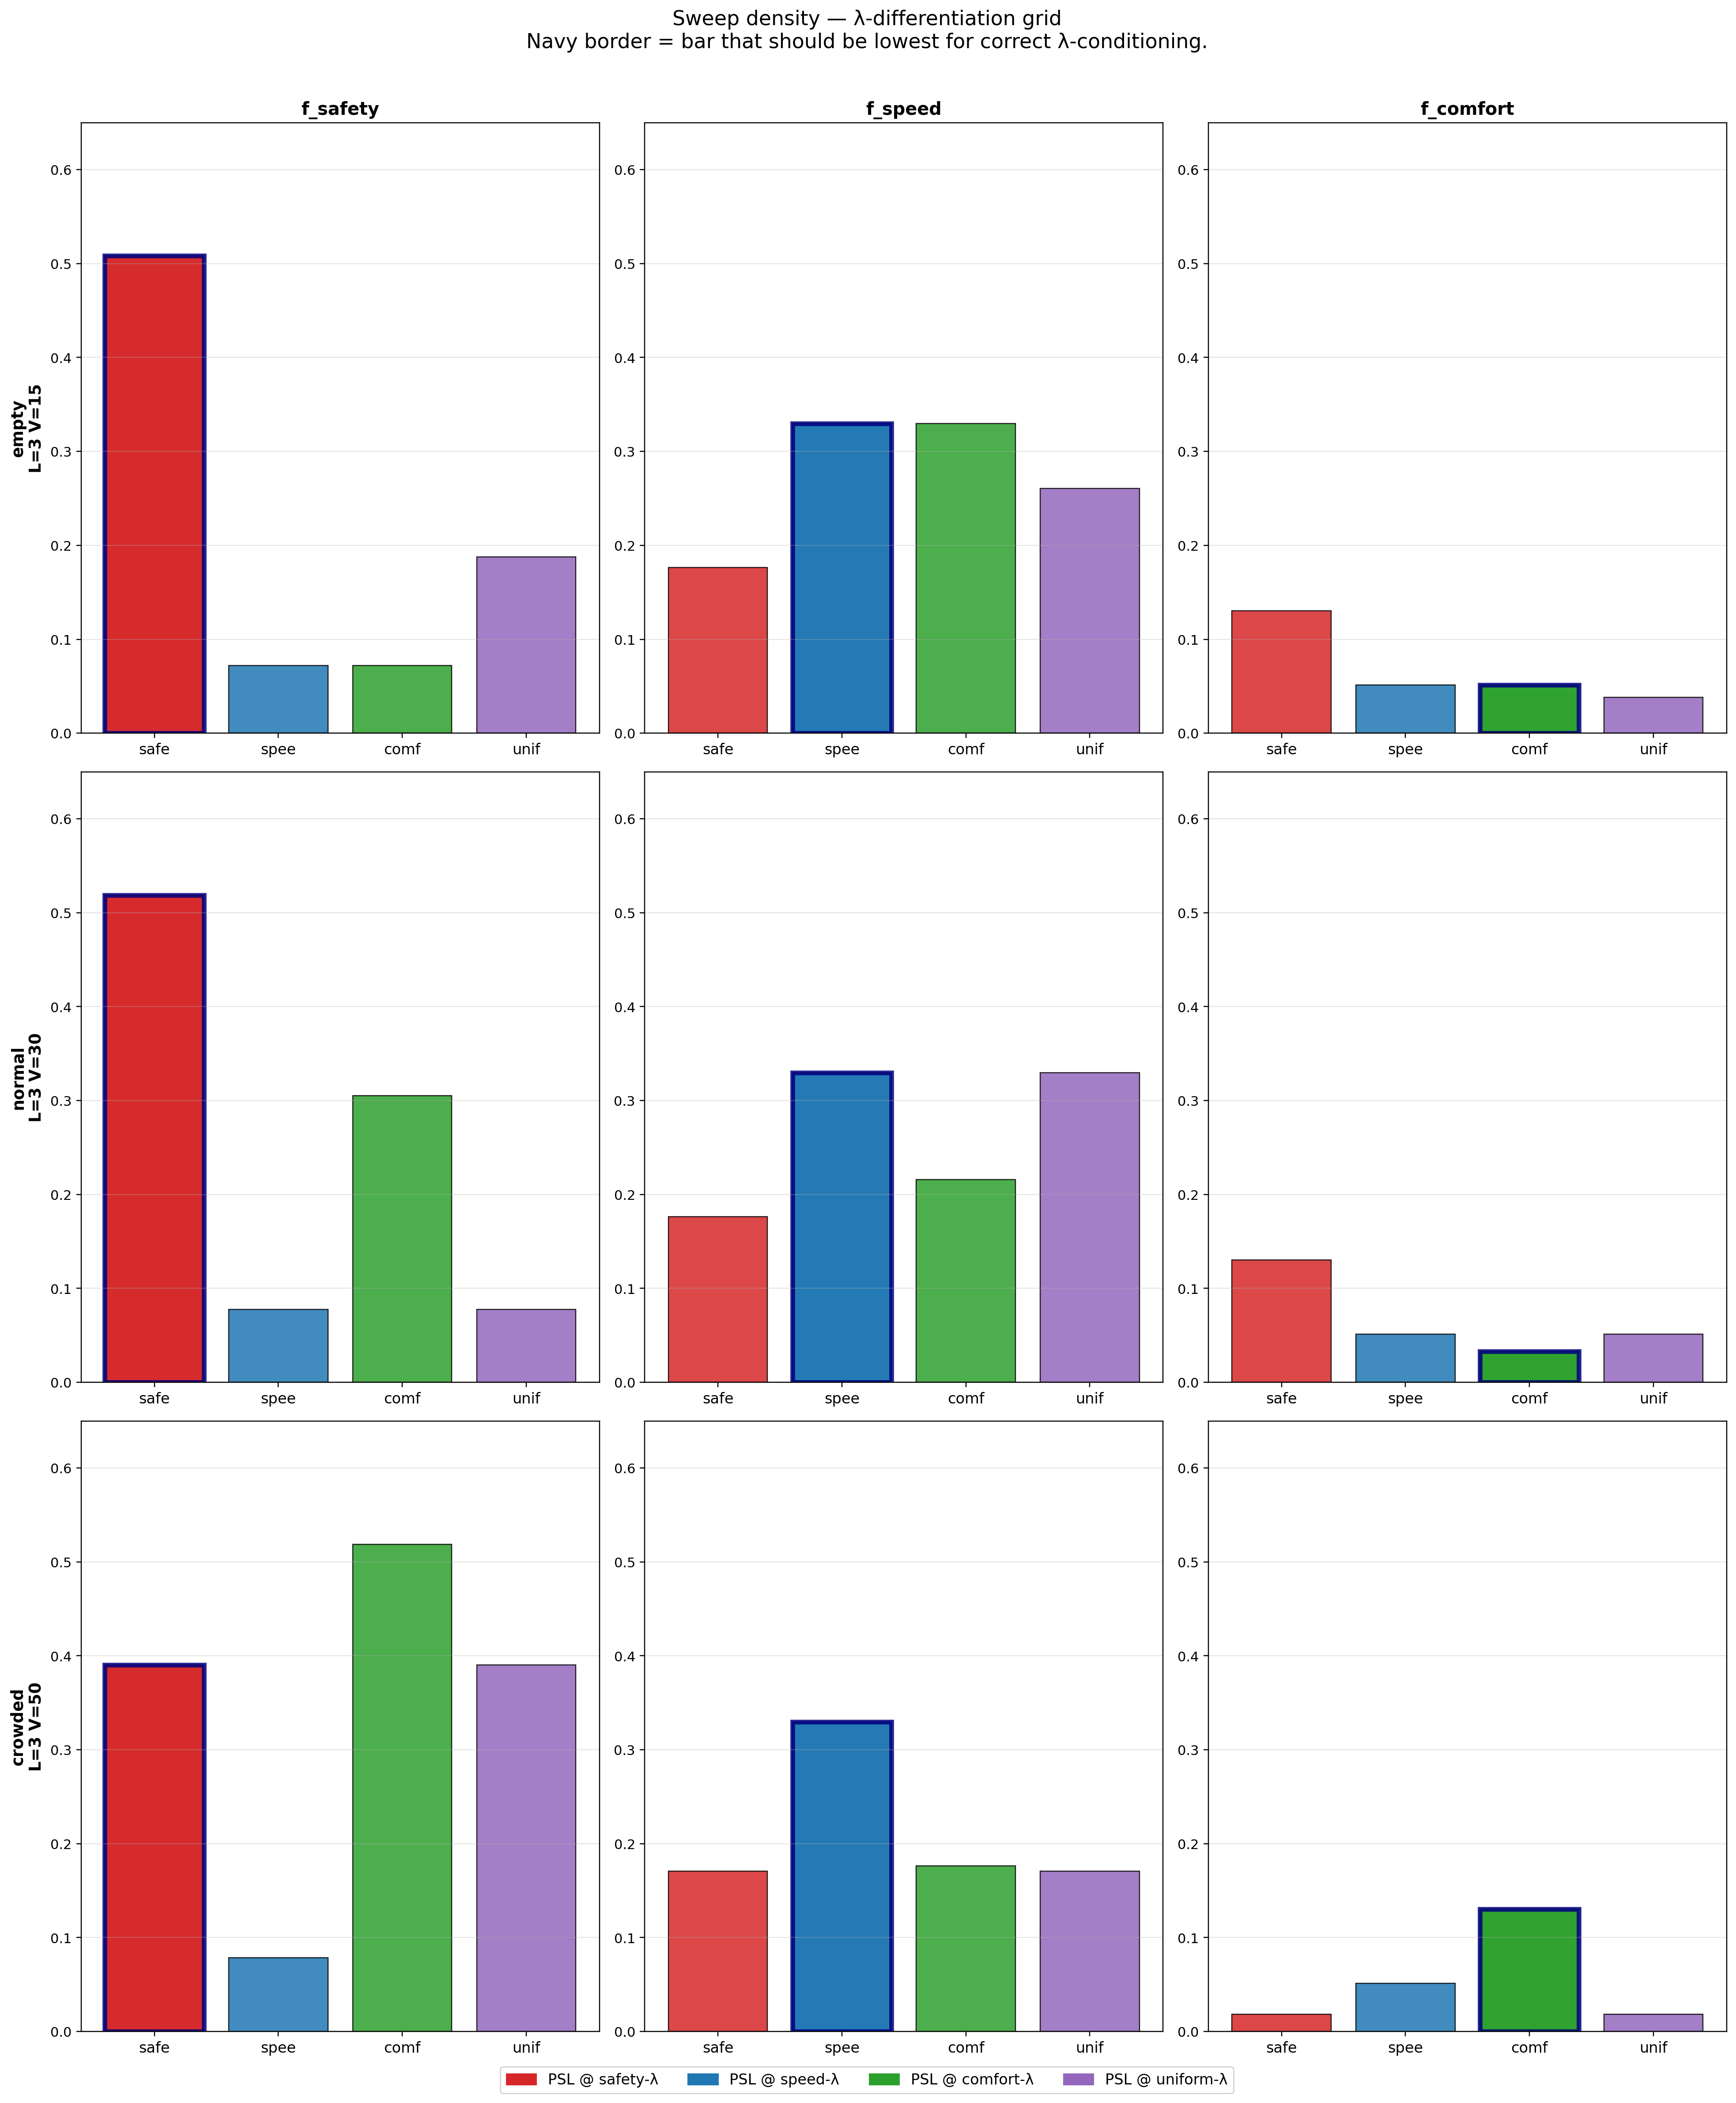
\includegraphics[width=\textwidth]{../checkpoints/exp4/lam_grid_density.png}
    \caption{Per-condition, per-objective bar charts for the four PSL preference variants. Rows correspond to traffic density conditions; columns to the three objectives. A navy border marks the ``owned'' objective for each preference (e.g.\ PSL @ $\lambda_s$ bar is navy-bordered in the $f_s$ column). Ideally the navy-bordered bar should be the shortest in its panel; this holds clearly for comfort in the normal condition but not for safety across all conditions.}
    \label{fig:lamgrid}
\end{figure}

\section{Discussion \& Conclusions}
\label{sec:discussion}

\subsection{Summary of Findings}

This project trained a preference-conditioned actor-critic via LibMOON's EPO solver on a multi-objective highway driving task and evaluated it against fixed-weight scalarized baselines across a traffic-density sweep.
Three primary conclusions emerge from the results.

\textbf{Partial preference responsiveness.}
The PSL policy demonstrates measurable preference conditioning for the comfort objective: in normal traffic, PSL @ $\lambda_c$ achieves $f_c = 0.033$ via a mixed IDLE/SLOWER strategy, outperforming the scalarized comfort baseline ($f_c = 0.097$) that commits to the suboptimal LANE\_LEFT action.
However, conditioning is inconsistent across preferences.
The safety preset $\lambda_s$ inadvertently reinforces aggressive lane-changing behaviour that increases collision risk rather than reducing it, because the safety surrogate monitors only the same-lane forward gap and cannot observe adjacent-lane hazards introduced by lane changes.
The speed preset $\lambda_v$ defaults to conservative SLOWER behaviour under the pressure of the absorbing crash penalty, failing to approach the speed performance of the FASTER-dominant scalarized baseline.

\textbf{EPO calibration was the critical algorithmic fix.}
The most impactful intervention was the EPO $v_k$ calibration override (Section~\ref{sec:challenges}).
Cumulative returns from crash episodes do not reveal the crash cost through the per-step recovery formula $G[t]-\gamma G[t+1]$, so EPO incorrectly treated safety as satisfied and directed gradient mass toward speed, sustaining a training-distribution spiral with crash rates near $60\%$ for over $200$ updates.
Overriding $v_{k,\text{safety}}=1.0$ for crashed episodes broke this spiral: crash rates fell to $25$--$35\%$ within $100$ updates, enabling the policy to learn non-trivial preference-conditioned behaviours.
The entropy annealing and advantage clipping interventions provided secondary stability benefits.

\textbf{Behavioural degeneracy limits Pareto coverage.}
Both PSL and scalarized baselines frequently collapse to single-action policies (SLOWER, FASTER, or IDLE).
The absorbing crash penalty creates a steep reward landscape that makes SLOWER the globally safe action and FASTER the globally fast action, leaving limited gradient signal in the interior of behaviour space.
As a result, multiple distinct preference vectors map to the same deterministic policy, narrowing the effective Pareto coverage achieved by the single trained PSL network.

\subsection{Limitations and Scope}

\textbf{Environment and objective simplifications.}
We work in a stylised highway environment with discrete meta-actions, perfect kinematic observations of five neighbours, and three simplified objectives.
Real-world autonomous driving contends with pedestrians, cyclists, traffic signals, partial and noisy sensing, varying road geometry, weather, and legal regulations that no simple preference vector captures \cite{kiran2021deep,hayes2022practical}.
The intent of this project is methodological --- to demonstrate that gradient-based MOO can produce preference-conditioned behaviour \emph{when the objectives are intuitive and the environment is tractable} --- rather than to make any claim about real-vehicle deployment.

\textbf{Same-lane-only safety surrogate.}
The iTTC and distance-violation terms observe only front vehicles in the ego's current lane.
Lane changes introduce adjacent-lane hazards invisible to the safety cost during training, which explains why PSL @ $\lambda_s$ learns to change lanes as a safety strategy yet incurs the highest $f_s$ among PSL variants.
Extending the surrogate to cover lateral conflict zones (e.g., a weighted combination of same-lane forward TTC and adjacent-lane merge TTC) would be the single highest-leverage improvement.

\textbf{Absorbing crash penalty dominates the landscape.}
A penalty of $1/(1-\gamma)\approx 33.3$ dwarfs typical per-episode returns of $5$--$8$ per objective.
While necessary to make crash avoidance the global optimum, it compresses the gradient signal in the non-crash regime and pushes most policies toward conservative SLOWER behaviour.
A smaller penalty paired with a shaped intermediate speed reward may allow richer trade-off learning without sacrificing crash aversion.

\textbf{Conditioning mechanism.}
We adopted preference-conditioned policies for stability rather than a true hypernetwork \cite{navon2020learning,liu2025pareto}.
Hypernetworks offer in principle stronger $\lambda$-dependence because they generate policy weights from $\lambda$, but were unstable under stochastic-RL gradients in our pilot experiments.

\subsection{Conclusions}

Gradient-based multi-objective optimisation (LibMOON's EPO) can be integrated with preference-conditioned actor-critic RL to produce partial Pareto-set learning on a stylised highway driving task.
The combination of deep $\lambda$ injection, preference magnitude scaling, smooth safety surrogate, and EPO $v_k$ re-calibration was collectively necessary: removing any one component either caused policy collapse or sustained high crash rates through training.
Among the three objectives, \emph{comfort conditioning is the clearest success}; safety conditioning requires a multi-lane-aware surrogate to avoid the lane-change trap; and speed conditioning requires a weaker crash penalty or explicit speed shaping to compete with the FASTER-dominant scalarized baseline.

The broader methodological takeaway is that gradient-based MOO solvers like EPO transfer to multi-objective RL, but require two non-obvious safeguards: (i) the per-step cost vector passed to the LP solver must accurately reflect episode-level consequences (not be contaminated by terminal effects that the cost-recovery formula cannot see), and (ii) the reward landscape must not collapse all preferences into a single dominant behaviour mode through an overly large absorbing penalty.

\section{Future Scope}
\label{sec:future}

\subsection{Richer \texttt{highway-env} Topologies}
The \texttt{highway-env} suite \cite{leurent2018highway} ships several environments beyond the open-highway setting we used. Each exercises different aspects of the safety/speed/comfort trade-off and would constitute a natural test of how much $\lambda$-dependent behaviour transfers across topology:
\begin{itemize}
    \item \textbf{\texttt{merge-v0}.} A merging on-ramp that demands explicit gap negotiation. Safety-leaning preferences should yield longer wait times before merging; speed-leaning preferences should accept smaller gaps. Lane-change events become the central cost driver, raising comfort's relevance compared to straight-line cruising.
    \item \textbf{\texttt{roundabout-v0}.} Continuous-yaw negotiation around a circular junction. Lateral acceleration becomes a first-class cost (the bicycle-model term we currently report grows with $v^2 / R$), and conflict points are dense -- a strong testbed for safety conditioning.
    \item \textbf{\texttt{intersection-v0}.} Multi-vehicle right-of-way decisions at a four-way junction. Tail-event safety metrics dominate here: collision rates per crossing maneuver are the natural KPI rather than mean iTTC.
    \item \textbf{\texttt{racetrack-v0}.} Curvy-road scenarios with continuous steering. Lateral acceleration is non-trivial to control even at modest speeds, decoupling the comfort objective from the binary lane-change events of the highway setting.
    \item \textbf{\texttt{parking-v0}.} Goal-conditioned low-speed manoeuvring. Comfort and precision (proximity to target pose) become the dominant objectives; safety appears in a different form (avoiding obstacles rather than keeping TTC).
\end{itemize}
Sweeping the same PSL recipe across these topologies would test whether the preference-conditioned representation generalises -- a much stronger claim than convergence on a single environment.

\subsection{Algorithmic Extensions}
\begin{itemize}
    \item \textbf{Continuous control.} Replace \texttt{DiscreteMetaAction} with a low-level continuous controller and a Gaussian policy. The $\lambda$-conditioning task would then have to discriminate between continuous behaviours rather than five discrete options, which is both harder and more directly applicable to real systems.
    \item \textbf{Hypernetwork revisit.} The collapse problem we documented in Section~\ref{sec:challenges} could be revisited under a true hypernetwork formulation, possibly stabilised through gradient surgery techniques \cite{sener2018multitask,lin2019pareto} or through curriculum-style preference scheduling.
    \item \textbf{Beyond linear scalarisation hulls.} Many candidate Pareto points for non-convex fronts are unreachable by linear scalarisation. Comparing EPO directly against pure linear scalarisation on a controlled non-convex synthetic objective would clarify how much of the Pareto front each method recovers in this setting \cite{boyd2004convex,roijers2013survey}.
    \item \textbf{Multi-agent and human-in-the-loop.} Heavy traffic in our setup is realised through scripted drivers (IDM/MOBIL); enabling multiple PSL-controlled agents with potentially different $\lambda$ would surface preference-incompatibility dynamics that single-agent PSL cannot expose.
\end{itemize}

\subsection{Theoretical Investigation}
The relationship between Dirichlet sampling concentration, EPO mixing weights, and policy collapse appears largely empirical in our work. Formal analysis -- e.g., conditions under which EPO's $\bm{\alpha}$ degenerates to a $\lambda$-independent direction given certain Jacobian structures -- would convert the heuristic interventions of Section~\ref{sec:challenges} into provable guarantees.

\begin{thebibliography}{20}

\bibitem{kiran2021deep}
B. R. Kiran, I. Sobh, V. Talpaert, P. Mannion, A. A. Al Sallab, S. Yogamani, and P. Pérez,
\textit{Deep Reinforcement Learning for Autonomous Driving: A Survey},
IEEE Transactions on Intelligent Transportation Systems, vol. 23, no. 6, pp. 4909-4926, 2022.

\bibitem{konda2000actor}
V. R. Konda and J. N. Tsitsiklis,
\textit{Actor-Critic Algorithms},
Advances in Neural Information Processing Systems 12 (NeurIPS 1999), 2000.

\bibitem{agbaje2024neuroaction}
O. Agbaje, Y. Jin, and M. Olusanya,
\textit{NeuroAction: a neuroevolutionary approach to reinforcement learning for autonomous vehicles},
Scientific Reports, vol. 14, no. 1, p. 11151, 2024.

\bibitem{hayes2022practical}
C. F. Hayes, R. Rădulescu, E. Bargiacchi, J. Källström, M. Macfarlane, M. Reymond, T. Verstraeten et al.,
\textit{A Practical Guide to Multi-Objective Reinforcement Learning and Planning},
Autonomous Agents and Multi-Agent Systems, vol. 36, no. 1, art. 2, 2022.

\bibitem{deb2002fast}
K. Deb, A. Pratap, S. Agarwal, and T. Meyarivan,
\textit{A Fast and Elitist Multiobjective Genetic Algorithm: NSGA-II},
IEEE Transactions on Evolutionary Computation, vol. 6, no. 2, pp. 182-197, 2002.

\bibitem{navon2020learning}
A. Navon, A. Shamsian, G. Chechik, and E. Fetaya,
\textit{Learning the Pareto Front with Hypernetworks},
International Conference on Learning Representations (ICLR), 2021.

\bibitem{liu2025pareto}
E. Liu, Y.-C. Wu, X. Huang, C. Gao, R.-J. Wang, K. Xue, and C. Qian,
\textit{Pareto Set Learning for Multi-Objective Reinforcement Learning},
Proceedings of the AAAI Conference on Artificial Intelligence, 2025.

\bibitem{zhang2024libmoon}
X. Zhang, L. Zhao, Y. Yu, X. Lin, Y. Chen, H. Zhao, and Q. Zhang,
\textit{LibMOON: A Gradient-based MultiObjective OptimizatioN Library in PyTorch},
Advances in Neural Information Processing Systems 37 (NeurIPS 2024), 2024.

\bibitem{leurent2018highway}
E. Leurent,
\textit{An Environment for Autonomous Driving Decision-Making},
GitHub repository, 2018. [Online]. Available: \url{https://github.com/Farama-Foundation/HighwayEnv}.

\bibitem{roijers2013survey}
D. M. Roijers, P. Vamplew, S. Whiteson, and R. Dazeley,
\textit{A Survey of Multi-Objective Sequential Decision-Making},
Journal of Artificial Intelligence Research, vol. 48, pp. 67-113, 2013.

\bibitem{vogel2003ttc}
K. Vogel,
\textit{A Comparison of Headway and Time to Collision as Safety Indicators},
Accident Analysis \& Prevention, vol. 35, no. 3, pp. 427-433, 2003.

\bibitem{rajamani2011vehicle}
R. Rajamani,
\textit{Vehicle Dynamics and Control}, 2nd ed.,
Springer Science \& Business Media, 2011.

\bibitem{abels2019dynamic}
A. Abels, D. M. Roijers, T. Lenaerts, A. Nowé, and D. Steckelmacher,
\textit{Dynamic Weights in Multi-Objective Deep Reinforcement Learning},
Proceedings of the 36th International Conference on Machine Learning (ICML), pp. 11-20, 2019.

\bibitem{mnih2016a3c}
V. Mnih, A. P. Badia, M. Mirza, A. Graves, T. Harley, T. P. Lillicrap, D. Silver, and K. Kavukcuoglu,
\textit{Asynchronous Methods for Deep Reinforcement Learning},
Proceedings of the 33rd International Conference on Machine Learning (ICML), 2016.

\bibitem{boyd2004convex}
S. Boyd and L. Vandenberghe,
\textit{Convex Optimization},
Cambridge University Press, 2004.

\bibitem{desideri2012mgda}
J.-A. Désidéri,
\textit{Multiple-gradient descent algorithm (MGDA) for multiobjective optimization},
Comptes Rendus Mathématique, vol. 350, no. 5-6, pp. 313-318, 2012.

\bibitem{sener2018multitask}
O. Sener and V. Koltun,
\textit{Multi-Task Learning as Multi-Objective Optimization},
Advances in Neural Information Processing Systems 31 (NeurIPS 2018), 2018.

\bibitem{lin2019pareto}
X. Lin, H.-L. Zhen, Z. Li, Q.-F. Zhang, and S. Kwong,
\textit{Pareto Multi-Task Learning},
Advances in Neural Information Processing Systems 32 (NeurIPS 2019), 2019.

\bibitem{mahapatra2020epo}
D. Mahapatra and V. Rajan,
\textit{Multi-Task Learning with User Preferences: Gradient Descent with Controlled Ascent in Pareto Optimization},
Proceedings of the 37th International Conference on Machine Learning (ICML), 2020.

\bibitem{perez2018film}
E. Perez, F. Strub, H. de Vries, V. Dumoulin, and A. Courville,
\textit{FiLM: Visual Reasoning with a General Conditioning Layer},
Proceedings of the AAAI Conference on Artificial Intelligence, 2018.

\end{thebibliography}

\end{document}